%% Theorie.tex
%%
%\usepackage[ngerman]{babel}
%% ==============
\chapter{Theoretische Grundlagen}
\label{ch:Theorie}
%% ==============

{\bibliographystyle{babalpha-fl}}	% german style

Das Standardmodell der Teilchenphysik beschreibt die bisher bekannten fundamentalen Bausteine der Materie sowie deren Wechselwirkungen. In Kapitel \ref{ch:Theorie:sec:Standardmodell} wird ein kurzer \"Uberblick \"uber das Standardmodell der Teilchenphysik gegeben, woraufhin in Abschnitt \ref{ch:Theorie:sec:ttH} genauer auf die Produktion von Higgs-Bosonen und Topquarks eingegangen wird.\\


%% ===========================
\section{Das Standardmodell der Teilchenphysik}
\label{ch:Theorie:sec:Standardmodell}
%% ===========================

Der folgende Abschnitt soll einen kurzen \"Uberblick \"uber das Standardmodell der Elementarteilchenphysik geben, dabei folgt er meist den Erkl\"arungen aus \cite{SWB-39819646X}.

Das Standardmodell der Elementarteilchenphysik ist eine Quantenfeldtheorie, die die Theorie der elektroschwachen Wechselwirkung mit der Quantenchromodynamik zusammenfasst. Die Materie des Universums besteht aus einigen grundlegenden Bausteinen, die durch vier elementare Kr\"afte beeinflusst werden \cite{O'Luanaigh:1997201}. Die bislang beste Beschreibung dieses Aufbaus liefert das Standardmodell, wenngleich es die vierte Kraft, die Gravitation, nicht erkl\"aren kann. Dennoch war es mit diesem Modell m\"oglich fast alle experimentellen Ergebnisse zu best\"atigen, sowie sehr pr\"azise Vorhersagen \"uber verschiedene Ph\"anomene zu treffen.

Die elementaren Kr\"afte, die im Standardmodell beschrieben sind, sind starke und schwache Wechselwirkung sowie die elektromagnetische Wechselwirkung. Der elektromagnetischen Wechselwirkung unterliegen alle Teilchen, die eine elektrische Ladung tragen. Die Ladung der schwachen Wechselwirkung wird schwache Ladung genannt, die der starken Wechselwirkung in Analogie zur Farbmischung, bei der sich drei verschiedene Ladungen (rot, gr\"un und blau) zur neutralen Ladung addieren (bei der Farbmischung wei\ss), Farbladung.

Die bislang entdeckte Materie besteht aus zwei Arten von Elementarteilchen, den Leptonen sowie den Quarks. Diese lassen sich jeweils in drei Familien unterteilen. Jede Quark-Familie besteht jeweils aus einem Quarkpaar und deren Antiteilchen, diese sind Up- und Down-, Strange- und Charm- sowie Bottom- und Topquark. Sie tragen sowohl elektrische, schwache und Farbladung und unterliegen damit allen vier Kr\"aften.\\
Leptonen bilden jeweils zusammen mit dem dazugeh\"origen Neutrino und den jeweiligen Antiteilchen eine Familie. Im Gegensatz zu den Quarks tragen Leptonen keine Farbladung und unterliegen damit nicht der starken Wechselwirkung. Neutrinos sind au\ss erdem elektrisch neutral, wodurch sie nur schwach wechselwirken.\\
Die Wechselwirkungen sind in ihrer Struktur sehr \"ahnlich und werden durch den Austausch von Vektorbosonen vermittelt. Diese sind die Gluonen der starken Wechselwirkung, die W- und Z-Bosonen der schwachen Wechselwirkung und die Photonen der elektromagnetischen. W\"ahrend die Fermionen, aus denen die Materie besteht, einen halbzahligen Spin besitzen, haben die Bosonen einen ganzzahligen Spin.

Der letzte fehlende Baustein im Standardmodell ist ein elementares Spin-0-Teilchen, ohne das keine konsistente Erkl\"arung f\"ur die W- und Z$^0$-Massen m\"oglich w\"are. Dieses ist das Higgs-Boson, welches 2012 am CERN entdeckt wurde. Die Kopplung zwischen Higgs-Boson und anderen Elementarteilchen ist proportional zur Fermionenmasse. In Abbildung \ref{fig:Standardmodell} sind alle elementaren Bosonen und Fermionen dargestellt.

\begin{figure}[hhh]
 \begin{center}
   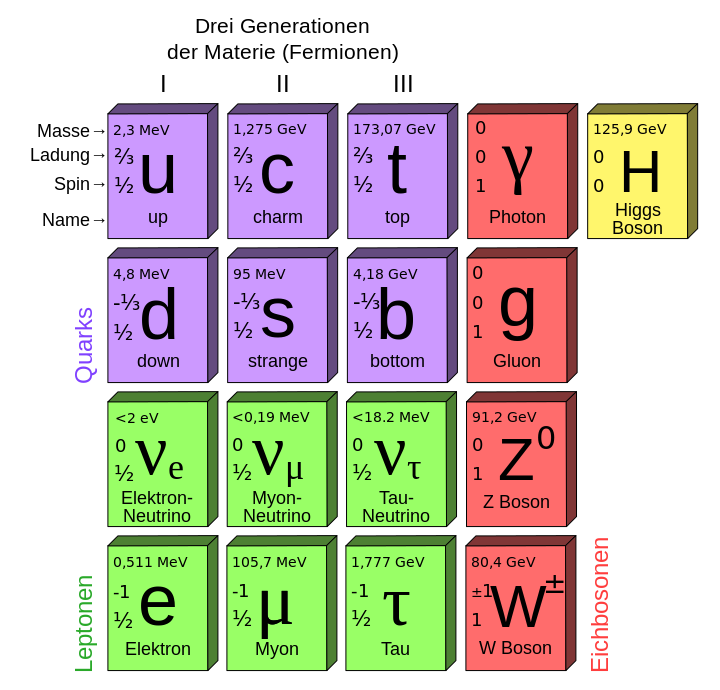
\includegraphics[width=\textwidth]{graphics/Standard_Model.png}
   \parbox[b]{12cm}{
     \caption[Standardmodell der Teilchenphysik]
             {\label{fig:Standardmodell} \it\!Die 12 fundamentalen Fermionen und f\"unf fundamentalen Bosonen des Standardmodells der Teilchenphysik \cite{wiki:Standardmodell}}
   }
 \end{center}
\end{figure}

Insgesamt stimmen die experimentellen Ergebnisse gut mit den Vorhersagen des Standardmodells \"uberein. Dennoch reicht das Modell nicht aus, um s\"amtliche Ph\"anomene zu erkl\"aren. Im Modell werden beispielsweise masselose Neutrinos gefordert, allerdings wird zur Erkl\"arung der beobachteten Neutrinooszillationen die Existenz massiver Neutrinos ben\"otigt.

%% ===========================
\section{Assoziierte Higgs-Boson-Top-Quark-Paar-Produktion (\ttH)}
\label{ch:Theorie:sec:ttH}
%% ===========================

Die Yukawa-Kopplungen sind im Standardmodell freie Parameter, die experimentell bestimmt werden m\"ussen. Da sie von den Fermionenmassen abh\"angen, ist eine Untersuchung der Kopplung zwischen Top-Quark und Higgs-Boson aufgrund der hohen Masse des Top-Quarks verglichen mit anderen Quarkmassen, besonders interessant. In Tabelle \ref{tab:quarkmasse} sind die Quarkmassen aufgelistet.\\


\begin{table}[hhh]\parbox{12cm}{
  \caption[Quarkmassen]{\it\!Quarkmassen {\rm \cite{Agashe:2014kda}}
  }\label{tab:quarkmasse}}
  \begin{center}
  \begin{tabular}{lll}
  \hline
  {\bf Quark} & {\bf Symbol} & {\bf Masse}  \\
  \hline \hline
     Up		& u & $\num{2,3}^{{+0,7}}_{{-0,5}}\si{\mega\electronvolt}$ \\
     Down	& d & $\num{4,8}^{{+0,5}}_{{-0,3}}\si{\mega\electronvolt}$ \\
     Strange& s & $\num{95}\pm \num{5}\si{\mega\electronvolt}$ \\
     Charm	& c & $\num{1,275}\pm \num{0,025}\si{\giga\electronvolt}$ \\ 
  	 Bottom & b & $\num{4,18}\pm \num{0,03}\si{\giga\electronvolt}$ \\
     Top    & t & $\num{173,07}\pm \num{0,52}\pm \num{0,72}\si{\giga\electronvolt}$ \\                                   
  \hline
  \end{tabular}
  \end{center}
\end{table}

Diese Kopplung kann im Prozess der assoziierten Produktion eines Higgs-Bosons mit einem Paar aus Top-Quark und Top-Anti-Quark untersucht werden.\\
Wechselwirkungen zwischen Teilchen k\"onnen durch Feynman-Diagramme visualisiert werden. In Abbildung \ref{fig:ttH_feynmans} sind exemplarisch einige Feynman-Diagramme zur \ttH-Produktion in f\"uhrender Ordnung abgebildet und zum Vergleich das Feynman-Diagramm der Gluon-Gluon-Fusion, des dominierenden Kanals der Higgs-Boson-Produktion am LHC, in Abbildung \ref{fig:gluonfusion}.

\begin{figure}[hhh]
 \begin{center}
   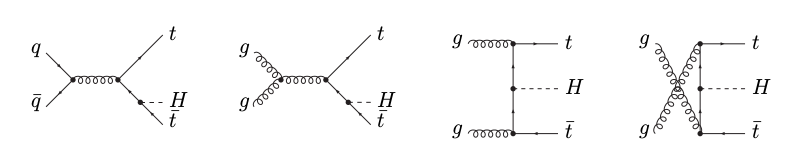
\includegraphics[width=\textwidth]{graphics/ttH_feynmans.png}
   \parbox[b]{12cm}{
     \caption[\ttH Feynman-Diagramme]
             {\label{fig:ttH_feynmans} \it\!Feynman-Diagramme f\"ur die \ttH-Produktion aus Hadronenkollisionen in f\"uhrender Ordnung \cite{hep-ph/0211352}}
   }
 \end{center}
\end{figure}

\begin{figure}[hhh]
 \begin{center}
   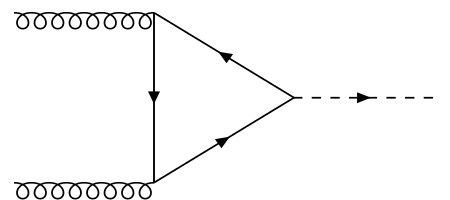
\includegraphics[width=0.4\textwidth]{graphics/gluonfusion.png}
   \parbox[b]{12cm}{
     \caption[Gluon-Gluon-Fusion Feynman-Diagramm]
             {\label{fig:gluonfusion} \it\!Feynman-Diagramm f\"ur die Gluon-Gluon-Fusion, den dominierenden Kanal der Higgs-Boson-Produktion am LHC, erstellt mit \cite{feynman_draw}}
   }
 \end{center}
\end{figure}